\documentclass[11pt,a4paper]{article}
\usepackage[utf8]{inputenc}
\usepackage[vietnamese]{babel}
\usepackage{amsmath,amssymb}
\usepackage[version=4]{mhchem}
\usepackage{geometry}
\geometry{top=1.5cm,bottom=1.2cm,left=1.4cm,right=1.4cm,headheight=28pt,headsep=12pt,footskip=18pt}
\usepackage{graphicx}
\usepackage{xcolor}
\usepackage{tabularx}
\usepackage{array}
\usepackage{colortbl}
\usepackage{tikz}
\usepackage{fancyhdr}
\usepackage{enumitem}
\usepackage{multido}
\usepackage{tcolorbox}

\definecolor{hfRed}{HTML}{D32F2F}
\definecolor{hfGreen}{HTML}{8BC390}
\definecolor{mainGreen}{HTML}{2E7D32}
\definecolor{solBlue}{HTML}{1565C0}
\definecolor{tableGreen}{HTML}{E8F5E9}

\usepackage{ex_test}

\pagestyle{fancy}
\fancyhf{}
\renewcommand{\headrulewidth}{0.75pt}
\renewcommand{\headrule}{\hbox to\headwidth{\color{hfGreen}\leaders\hrule height \headrulewidth\hfill}}
\renewcommand{\footrulewidth}{0.75pt}
\renewcommand{\footrule}{\hbox to\headwidth{\color{hfGreen}\leaders\hrule height \footrulewidth\hfill}}

\fancyhead[L]{\small\itshape\color{hfRed}Tài liệu lưu hành nội bộ}
\fancyhead[R]{\small\color{hfRed}Thầy \textbf{TRẦN VĂN THẠNH} - 0777.470.803}

\fancyfoot[L]{\footnotesize\itshape\color{hfRed}CS1: 6/15 Nguyễn Hoàng, P. Kim Long, TP Huế \quad|\quad CS2: 24 Đặng Thái Thân, TP Huế}
\fancyfoot[R]{\small\textbf{\color{hfRed}Trang \thepage}}

\setlength{\parindent}{0pt}
\setlength{\parskip}{2pt}

\begin{document}

\begin{minipage}[t]{0.48\textwidth}
\textbf{SỞ GIÁO DỤC VÀ ĐÀO TẠO}\\
\textbf{TRƯỜNG THPT CAO THẮNG}\\
\textit{ĐỀ CHÍNH THỨC}\\
\textit{(Đề thi có 03 trang)}
\end{minipage}
\hfill
\begin{minipage}[t]{0.48\textwidth}
\raggedleft
\textbf{\color{hfRed}ĐỀ KIỂM TRA CUỐI KÌ 1}\\
\textbf{NĂM HỌC 2025 -- 2026}\\
\textbf{MÔN: HÓA HỌC 12}\\
\textit{Thời gian làm bài: 45 phút (không kể thời gian phát đề)}\\
\textbf{MÃ ĐỀ: 1203}
\end{minipage}

\vspace{4pt}
\noindent
\textit{Họ và tên:} \dotfill \textit{Số báo danh:} \dotfill

\vspace{3pt}
\noindent
\textit{\footnotesize Cho biết: $\ce{H}=1;\ \ce{C}=12;\ \ce{N}=14;\ \ce{Cl}=35,5;\ \ce{O}=16$.}

\vspace{3pt}
\hrule color{hfGreen} height 0.5pt

\vspace{4pt}
\noindent
{\color{mainGreen}\textbf{\Large I. PHẦN TRẮC NGHIỆM (7,0 ĐIỂM)}}

\vspace{3pt}
\noindent
{\color{mainGreen}\textbf{\large PHẦN I. Câu trắc nghiệm nhiều phương án lựa chọn.}}\\
\textit{\small Thí sinh trả lời từ câu 1 đến câu 12. Mỗi câu hỏi thí sinh chỉ chọn một phương án.}
\vspace{2pt}

\begin{ex}
Trong pin điện hoá, quá trình khử
\choice
{không xảy ra ở cả cực âm và cực dương}
{\True xảy ra ở cực dương}
{xảy ra ở cực âm}
{xảy ra ở cực âm và cực dương}
\end{ex}
\begin{ex}
Glucose là chất dinh dưỡng và được dùng làm thuốc tăng lực cho người già, trẻ em và người ốm. Số nguyên tử oxygen trong phân tử glucose là
\choice
{12}
{\True 6}
{11}
{5}
\end{ex}
\begin{ex}
Quá trình cộng hợp liên tiếp nhiều phân tử nhỏ giống nhau hoặc tương tự nhau (monomer) tạo thành phân tử lớn (polymer) được gọi là phản ứng
\choice
{xà phòng hoá}
{thuỷ phân}
{trùng ngưng}
{\True trùng hợp}
\end{ex}
\begin{ex}
Poly(methyl methacrylate) là chất rắn trong suốt, có khả năng cho ánh sáng truyền qua tốt nên được dùng để chế tạo thuỷ tinh hữu cơ. Poly(methyl methacrylate) được điều chế từ monomer nào sau đây?
\choice
{$\ce{CH3COOC(CH3)=CH2}$}
{$\ce{CH3COOCH=CH2}$}
{$\ce{CH2=CHCOOCH3}$}
{\True $\ce{CH2=C(CH3)COOCH3}$}
\end{ex}
\begin{ex}
Polymer nào sau đây trong thành phần chỉ gồm hai nguyên tố C và H?
\choice
{Tơ nylon-6,6}
{Poly(methyl methacrylate)}
{Poly(phenol formaldehyde)}
{\True Polybuta-1,3-diene}
\end{ex}
\begin{ex}
Phát biểu nào sau đây là bản chất của sự lưu hoá cao su?
\choice
{\True Tạo cầu nối disulfide giữa các mạch phân tử cao su}
{Tạo loại cao su nhẹ hơn}
{Giảm giá thành cao su}
{Làm cao su dễ ăn khuôn}
\end{ex}
\begin{ex}
Trong các chất sau, chất nào là amin bậc II?
\choice
{$\ce{CH3-CH(CH3)-NH2}$}
{$\ce{C6H5NH2}$}
{\True $\ce{CH3-NH-CH3}$}
{$\ce{H2N-[CH2]6-NH2}$}
\end{ex}
\begin{ex}
Ở điều kiện chuẩn, thiết lập được điện cực zinc ($\ce{Zn}$) bằng cách nhúng thanh $\ce{Zn}$ vào dung dịch
\choice
{\True $\ce{ZnSO4}\ 1\text{ M}$}
{$\ce{H2SO4}\ 1\text{ M}$}
{$\ce{NaCl}\ 1\text{ M}$}
{$\ce{HCl}\ 1\text{ M}$}
\end{ex}
\begin{ex}
Trùng hợp propylene thu được polymer có tên gọi là
\choice
{\True polypropylene}
{polyethylene}
{polystyrene}
{poly(vinyl chloride)}
\end{ex}
\begin{ex}
Chất nào sau đây thuộc loại $\alpha$-amino acid?
\choice
{$\ce{H2NCH2CH2COOH}$}
{$\ce{HOCH2COOH}$}
{$\ce{H2NCH(CH3)NH2}$}
{\True $\ce{H2NCH(CH3)COOH}$}
\end{ex}
\begin{ex}
Chất hữu cơ $\ce{X}$ có nhiều trong cây mía, hoa thốt nốt, củ cải đường,... Nồng độ của $\ce{X}$ trong nước mía có thể đạt tới 13\%. Chất $\ce{X}$ là
\choice
{fructose}
{maltose}
{\True saccharose}
{glucose}
\end{ex}
\begin{ex}
Phát biểu nào sau đây không đúng?
\choice
{Tơ nylon-6,6 được điều chế bằng phản ứng trùng ngưng}
{Tơ nitron được điều chế bằng phản ứng trùng hợp}
{\True Tơ tằm thuộc loại tơ bán tổng hợp}
{Cao su lưu hóa có cấu trúc mạng không gian}
\end{ex}
\vspace{4pt}
\noindent
{\color{mainGreen}\textbf{\large PHẦN II. Câu trắc nghiệm đúng sai.}}\\
\textit{\small Thí sinh trả lời từ câu 1 đến câu 2. Trong mỗi ý a), b), c), d) ở mỗi câu, thí sinh chọn đúng hoặc sai.}
\vspace{2pt}

\begin{ex}
Cho các cặp oxi hóa - khử và thế điện cực chuẩn sau:
\begin{center}
\renewcommand{\arraystretch}{1.2}
\begin{tabular}{|c|c|c|c|c|c|}
\hline
\rowcolor{tableGreen}
\textbf{Cặp oxi hóa-khử} & $\ce{Zn^2+/Zn}$ & $\ce{Cu^2+/Cu}$ & $\ce{Fe^2+/Fe}$ & $\ce{Pb^2+/Pb}$ & $\ce{Fe^3+/Fe^2+}$ \\
\hline
$E^\circ\ (\text{V})$ & $-0,76$ & $0,34$ & $-0,44$ & $-0,13$ & $0,77$ \\
\hline
\end{tabular}
\end{center}
\choiceTF
{Cho $\ce{Zn}$ dư tác dụng với dung dịch $\ce{FeCl3}$ đến khi phản ứng hoàn toàn thu được dung dịch gồm $\ce{FeCl2}$ và $\ce{ZnCl2}$}
{\True Tính oxi hoá của $\ce{Fe^3+} > \ce{Cu^2+} > \ce{Pb^2+} > \ce{Fe^2+} > \ce{Zn^2+}$}
{\True Sức điện động chuẩn của pin $\ce{Fe-Cu}$ có giá trị là $0,78\text{ V}$}
{Cho kim loại $\ce{Fe}$ tác dụng với dung dịch $\ce{Cu(NO3)2}$ dư, đến khi phản ứng xảy ra hoàn toàn, thu được dung dịch gồm $\ce{Cu(NO3)2}$ và $\ce{Fe(NO3)3}$}
\end{ex}
\begin{ex}
Poly(vinyl chloride) (PVC) là chất dẻo có tính cách điện tốt, bền với acid, dùng phổ biến để sản xuất vật liệu cách điện, ống dẫn nước, áo mưa.
\begin{center}
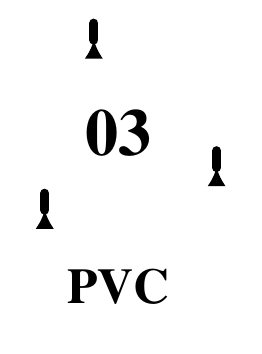
\includegraphics[width=2.0cm]{San_Pham/images_de1203/pvc_logo.png}
\end{center}
\choiceTF
{Poly(vinyl chloride) được điều chế từ vinyl chloride bằng phản ứng trùng ngưng}
{\True Cho sơ đồ chuyển hóa: $\ce{CH4 -> C2H2 -> C2H3Cl -> PVC}$. Để tổng hợp $250\text{ kg}$ PVC theo sơ đồ trên thì cần $396,64\text{ m}^3$ khí $\ce{CH4}$ (hiệu suất của cả quá trình là $50\%$)}
{\True Công thức của vinyl chloride là $\ce{CH2=CHCl}$}
{X kém bền với acid}
\end{ex}
\vspace{4pt}
\noindent
{\color{mainGreen}\textbf{\large PHẦN III. Câu trắc nghiệm trả lời ngắn.}}\\
\textit{\small Thí sinh trả lời từ câu 1 đến câu 4. Thí sinh điền kết quả vào ô trả lời tương ứng.}
\vspace{2pt}

\begin{ex}
Caprolactam được tổng hợp từ cuối thế kỉ XIX. Hiện nay, nhu cầu sản xuất caprolactam trên thế giới khoảng 10 triệu tấn/năm. 90\% trong đó dùng để tổng hợp tơ capron. Trong công nghiệp, caprolactam được điều chế theo sơ đồ sau:
\begin{center}
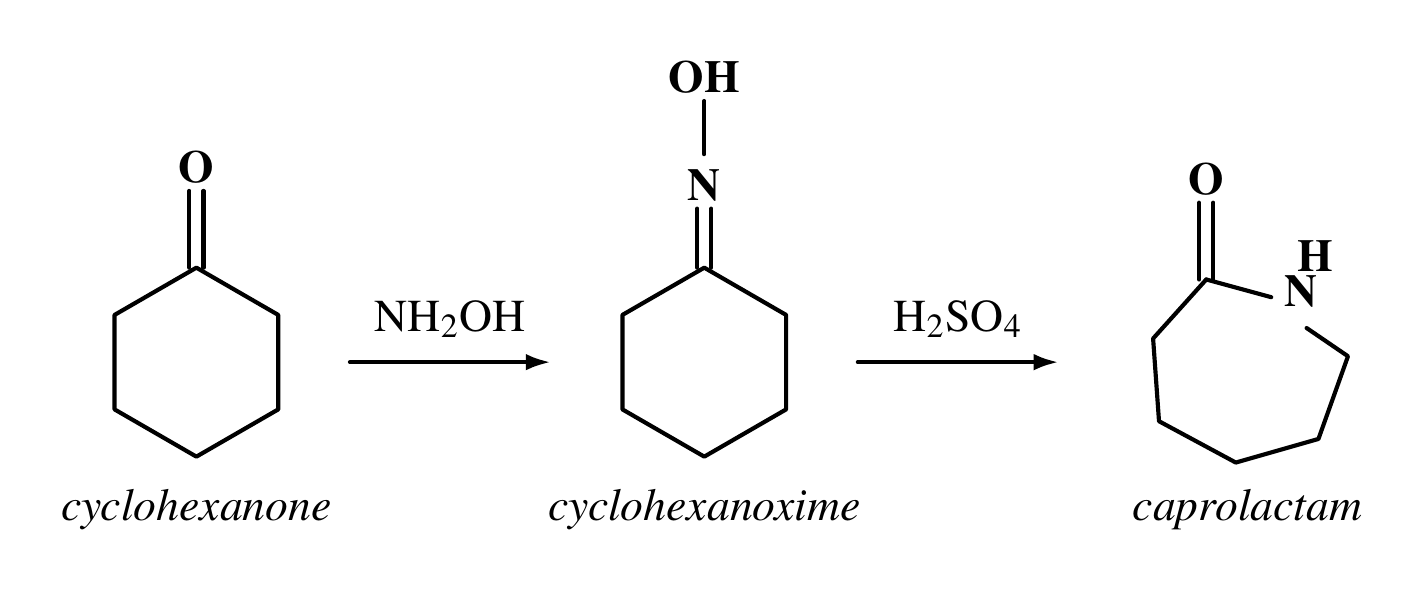
\includegraphics[width=13.5cm]{San_Pham/images_de1203/so_do_caprolactam.png}
\end{center}
Để sản xuất 10 triệu tấn caprolactam, cần sử dụng bao nhiêu triệu tấn cyclohexanone? Giả sử hiệu suất trung bình của cả quá trình trên là $60\%$. \textit{(Kết quả làm tròn đến hàng phần mười)}.
\hfill \textbf{Trả lời:} \dotfill
\end{ex}
\begin{ex}
Cho các nguyên liệu: dầu mỏ, acid béo, dầu thực vật, sodium hydroxide, sulfuric acid, mỡ động vật. Có bao nhiêu chất sử dụng được để điều chế xà phòng trực tiếp bằng phản ứng xà phòng hóa?
\hfill \textbf{Trả lời:} \dotfill
\end{ex}
\begin{ex}
Cho sơ đồ chuyển hóa sau (mỗi mũi tên là một phản ứng):\\
$\text{Tinh bột} \longrightarrow \ce{X} \longrightarrow \ce{Y} \longrightarrow \ce{Z} \longrightarrow \text{methyl acetate}$. Xác định phân tử khối của $\ce{Z}$.
\hfill \textbf{Trả lời:} \dotfill
\end{ex}
\begin{ex}
Khi thuỷ phân hoàn toàn $500\text{ gam}$ protein $\ce{X}$ thì thu được $178\text{ gam}$ alanine. Nếu phân tử khối của $\ce{X}$ là $50000$ thì số mắt xích alanine trong phân tử $\ce{X}$ là bao nhiêu?
\hfill \textbf{Trả lời:} \dotfill
\end{ex}
\vspace{4pt}
\noindent
{\color{mainGreen}\textbf{\Large II. PHẦN TỰ LUẬN (3,0 ĐIỂM)}}

\vspace{3pt}

\noindent
\textbf{Câu 1. (1,0 điểm)} Benzyl salicylate được sử dụng làm chất cố định hương nước hoa, các sản phẩm khử mùi, kem chống nắng... Chất này được điều chế bằng phản ứng giữa salicylic acid ($o$-hydroxy benzoic acid) và benzyl alcohol.\\
a. Viết phương trình hoá học của các phản ứng điều chế ester trên.\\
b. Để sản xuất $400\text{ lít}$ benzyl salicylate nguyên chất ($D = 1,17\text{ g/mL}$) thì cần tối thiểu bao nhiêu lít benzyl alcohol nguyên chất ($D = 1,04\text{ g/mL}$), biết hiệu suất phản ứng là $80\%$.

\vspace{2pt}
\multido{\i=1+1}{8}{\noindent\dotfill\\}

\vspace{4pt}
\noindent
\textbf{Câu 2. (1,0 điểm)} Trong số các loại tơ sau: tơ tằm, tơ visco, tơ nylon-6,6, len, tơ cellulose acetate, tơ capron.\\
a. Tơ nào là tơ tự nhiên, tơ nhân tạo và tơ tổng hợp?\\
b. Viết phương trình hoá học của phản ứng điều chế các loại tơ tổng hợp ở trên từ các monomer tương ứng (ghi rõ điều kiện nếu có).

\vspace{2pt}
\multido{\i=1+1}{8}{\noindent\dotfill\\}

\vspace{4pt}
\noindent
\textbf{Câu 3. (1,0 điểm)} Biết phản ứng oxi hoá - khử xảy ra trong một pin điện hoá: $\ce{Cu + 2Ag+ -> Cu^2+ + 2Ag}$.\\
a. Viết các quá trình xảy ra tại mỗi điện cực.\\
b. Cho thế điện cực chuẩn của các cặp $\ce{Zn^2+/Zn}$ và $\ce{Ag+/Ag}$ lần lượt là $-0,76\text{ V}$ và $0,8\text{ V}$. Sức điện động chuẩn của pin điện hoá $\ce{Zn-Cu}$ là $1,10\text{ V}$. Tính sức điện động chuẩn của pin điện hoá $\ce{Cu-Ag}$.

\vspace{2pt}
\multido{\i=1+1}{8}{\noindent\dotfill\\}

\vspace{8pt}
\begin{center}
\textbf{---------- HẾT ----------}
\end{center}

\end{document}
